\section{Background} \label{sect:2}

In this Section~I will deepen on the theoretical background required for the project. First, in Section~\ref{sect:2regularizers}, I will describe $\ell_1$ and $\ell_2$ norm regularization and common image regularizers like total variation ($\operatorname{TV}$), group sparsity and the Hessian-Schatten norm. Then, in Section~\ref{sect:2prox}, I will describe the proximal operator and some relevant optimization algorithms for image reconstruction. 

\subsection{Image Regularization}  \label{sect:2regularizers}

As mentioned in Section~\ref{sect:1}, sparsity is a well known property of real life images and objects. In particular, sparsity on transforms that measure variation in the vicinity of pixels (e.g., the wavelet transform \cite{vonesch_fast_2009}, or derivative operators \cite{soubies_pocket_2019, chambolle_image_1997}) promote smoothness on an image, and in many cases they are a good indicator of low noise and high fidelity with the true object. Moreover, the $\ell_1$ norm is a good objective function to promote sparsity, which is why common image regularizers are a combination of $\ell_1$ norms measuring a transform $\mathbf{L}$ that measures a property that is desired to be small.

Other desirable properties in image regularizers are convexity -to make optimization feasible- and  invariance to rotation, translation, and scaling, so that they do not depend on any specific coordinate axis. 

\noindent\textbf{$\mathbf{\ell_p}$ regularization} 

As aforementioned, $\ell_1$ and $\ell_2$ norms are common choices of $\operatorname{R}$ for regularization. When acting on a raw measurement, $\ell_p$ regularization consists in choosing the point within a validity region (which can be determined by a scaling parameter $\lambda$ multiplying $\mathcal{R}$ in \eqref{eq:imaging_problem}) that touches the smallest norm ball of the chosen $\ell_p$ norm. This is exemplified in Figure \ref{fig:l1_reg} (reused with permission from \cite{noauthor_tutorial_2020}) for the $\ell_1$ and $\ell_2$ norms.  
\begin{figure}[H]
  \begin{center}
  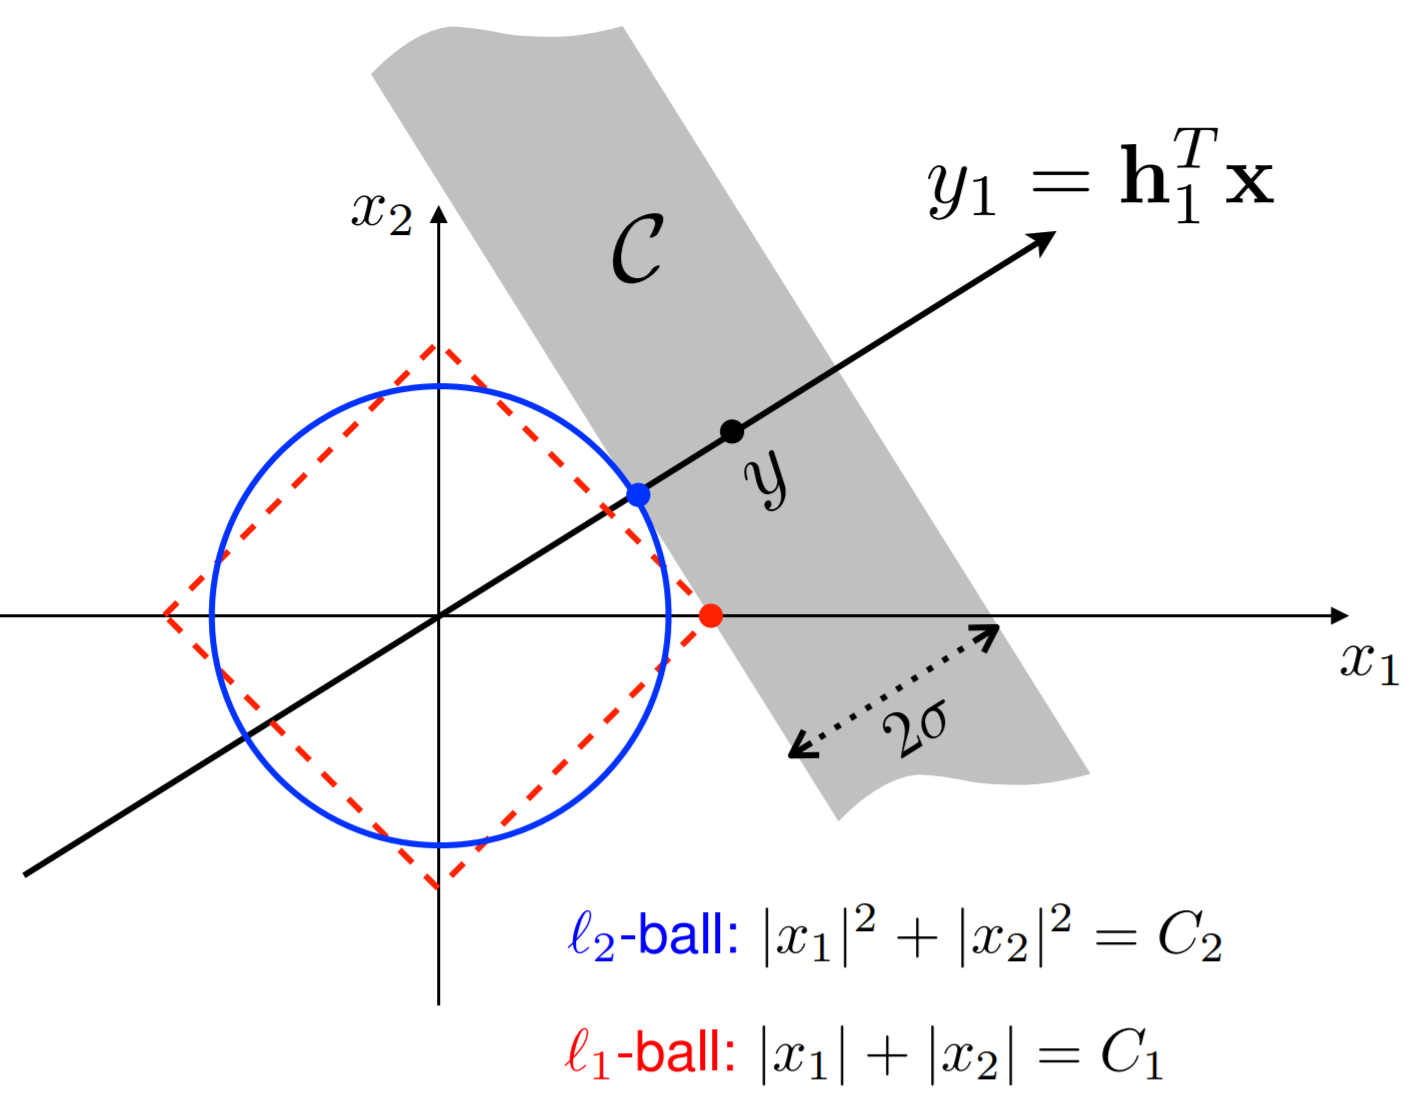
\includegraphics[width = 0.55
  \textwidth]{images/l1_reg.PNG}
  \caption{$\ell_1$ and $\ell_2$ norm regularization on a low dimensional example. The regularization of $\mathbf{x}$ consists in finding the points (in red for the $\ell_1$ norm and blue for the $\ell_2$ norm) as optimal reconstruction. The gray area corresponds to the data fidelity region. Figure reused with permission from \cite{noauthor_tutorial_2020}.}
  %$y_1$ (obtained from the sampling $\mathbf{h}_1^T\mathbf{x}$) results in choosing the points $x_1$ and $x_2$ within the data fidelity region (shaded in gray) that touch the smallest possible norm balls within this region. Figure taken from \cite{noauthor_tutorial_2020}.} 
  \label{fig:l1_reg}
  \end{center}
\end{figure}

In Figure \ref{fig:l1_reg}, in an example of a $2$-dimensional inverse problem, the properties of $\ell_1$ and $\ell_2$ regularization are exemplified. The solution of $\ell_2$ norm regularization lies within the space spanned by $\mathbf{h}_1^T$, but does not necessarily promote sparsity. On the other hand, $\ell_1$ regularization promotes sparsity in the solution -under some conditions in $\mathbf{h}_1^T$-.

\noindent\textbf{Group Sparsity}

In images where there is prior information on the structure of the image in the form of pixel labelling (e.g., many cell images where structural information can be known \cite{baritaux_sparsity-driven_2011}, or using a spatio-temporal representation of a single image \cite{del_aguila_pla_cell_2018-1, del_aguila_pla_cell_2018}), $\ell_p$ norm regularization can be applied independently (without overlap) to the different structures. This results in a vector of measurements of each region, and a second norm can be taken over this new vector. This technique has been proven to be successful in image reconstruction tasks, and is known as group sparsity. It is also referred to as $\|\cdot\|_{p, q}$ mixed-norm, and is formalized by
\begin{equation}
    \|\mathbf{x}\|_{p, q} = \left(\sum^S_{i = 1}\|\mathbf{x}_i\|_p^q\right)^\frac{1}{q},
    \label{eq:group_sparsity}
\end{equation}
where $S$ is the total number of groups, and $\mathbf{x}_i$ represents the $i^{th}$ group. In short, \eqref{eq:group_sparsity} shows that the $\ell_p$ norm is taken on the different groups individually, and the $\ell_q$ norm is taken across the group norms. The different groups $\mathbf{x}_i$ need not have the same size.  

\noindent\textbf{Total Variation \cite{chambolle_image_1997, chambolle_introduction_2009}}

Total variation ($\operatorname{TV}$) is a tool that has been used extensively in image reconstruction. It combines the gradient operator  $\mathbf{\nabla}_n = [\mathbf{D}_1, ..., \mathbf{D}_n]$ with the mixed $\|\cdot\|_{i,j}$ norm. In this context and applied to an image $\mathbf{x} \in \mathbb{R}^{N \times M}$, $\mathbf{\nabla}_2\mathbf{x} \in \mathbb{R}^{2\times N \times M}$ is a $3$-dimensional array, where the derivatives along the two original dimensions are stacked to form the third dimension. So, $i$ stands for the norm applied to $\mathbf{\nabla}_n$ along the $1^{\mathrm{st}}$dimension -along the values of the gradients in the same position-. After applying this norm, the result has the original dimensions of $\mathbf{x}$,  $\mathbb{R}^{N \times M}$. $j$ is then the norm applied to this matrix to result in a scalar. For example, $\operatorname{TV}$ with mixed $\|\cdot \|_{1, 1}$ norm is written explicitly as
\begin{equation}
    \mathcal{R}(\mathbf{x}) = \sum^N_{n = 1}\|\mathbf{D}_1\mathbf{x}\|_n + \|\mathbf{D}_2\mathbf{x}\|_n.
    \label{eq:tv11}
\end{equation}

In \eqref{eq:tv11} it is shown explicitly that 2 different transforms ($\mathbf{D}_\mathbf{1}$ and $\mathbf{D}_\mathbf{2}$) are taken. Inside the summation, the $\ell_1$ norm along the first dimension is taken by summing absolute values at each element $n$. The summation stands for the outer norm, taken over the resulting $\mathbb{R}^{N \times M}$ array. Of course this is equivalent to taking the $\ell_1$ norm over the original $\mathbb{R}^{2 \times N \times M}$ array, but the notation serves for illustration purposes. 

\eqref{eq:tv11} is sometimes referred to as nonanisotropic $\operatorname{TV}$, since it is not invariant to rotation. On the other hand, $\operatorname{TV}$ with mixed $\|\cdot \|_{2, 1}$ norm is referred to as isotropic $\operatorname{TV}$, as rotations in the coordinate axis do not affect solution of the minimization of the $\ell_2$ norm. It is  written explicitly as
\begin{equation}
    \mathcal{R}(\mathbf{x}) = \sum^N_{n = 1}\sqrt{[\mathbf{D_1x}]^2_n + [\mathbf{D_2x}]^2_n}.
    \label{eq:tv21}
\end{equation}

In  \eqref{eq:tv21}, it is necessary to write explicitly the two different norms. While this norm is invariant to rotation, its minimization is more complex than the minimization of the nonisotropic $\operatorname{TV}$, and in practice both produce good results. However, there are some limitations with $\operatorname{TV}$, regardless of the choice of $i, j$.  Since it promotes vanishing first order derivatives, the results are usually piece-wise constant, an effect that is known as \textit{staircase effect} (see for example, Figure \ref{fig:tv_experiment} in Section~\ref{sect:3}).  

\noindent\textbf{Hessian Schatten Norm}

As an alternative to $\operatorname{TV}$ and a solution for the staircase effect, the Hessian-Schatten norm was proposed in \cite{lefkimmiatis_hessian_2013}. Instead of using first order derivatives, it uses second order derivatives. It computes the $\|\cdot \|_{S_p, 1}$ norm of the Hessian operator $\mathbf{HS} = [\mathbf{D}_{i, j}]_{1\leq ij\leq}$ applied to $x\in \mathbb{R}^\mathrm{N}$
% \begin{equation}
%     \mathcal{R}(\mathbf{x}) = \sum^N_{n=1}\left\|\mathbf{HS}\right\|_{S_p} = \sum^N_{n = 1}\left\|
%   \begin{bmatrix}
%     [D_{11}\mathbf{x}]_n [D_{12}\mathbf{x}]_n\\
%     [D_{21}\mathbf{x}]_n [D_{22}\mathbf{x}]_n
%   \end{bmatrix}\right\|_{S_p}, 
%     \label{eq:hs}
% \end{equation}
\begin{equation}
    \mathcal{R}(\mathbf{x}) = \sum^N_{n = 1}\left\|
  \begin{bmatrix}
    [D_{11}\mathbf{x}]_n [D_{12}\mathbf{x}]_n\\
    [D_{21}\mathbf{x}]_n [D_{22}\mathbf{x}]_n
  \end{bmatrix}\right\|_{S_p}, 
    \label{eq:hs}
\end{equation}
where $\|\cdot \|_{S_p}$ denotes the Schatten norm. It is defined as
\begin{equation}
    \|\mathbf{X}\|_{S_p} = \left( \sum_{k=1}^{\min\left(n_{1},n_{2}\right)}\mathbf{\sigma}_{k}^{p}\left({\mathbf X}\right)\right)^\frac{1}{p}, 
    \label{eq:schatten_norm}
\end{equation}
where $\mathbf{\sigma}_{k}^{p}\left({\bf X}\right)$ denotes the $k_{\mathrm{th}}$ singular value of $\bf{X}$. 

In contrast to $\operatorname{TV}$, the use of second order derivatives results in piece-wise linear images, far more realistic than the piece-wise constant results of $\operatorname{TV}$. Moreover, the Hessian Schatten norm preserves the properties of convexity and invariance.

None of $\operatorname{TV}$ nor the Hessian Schatten norm are differentiable. However, their proximal operators can be taken efficiently, which means that the algorithm of choice for the optimization problem described in  \eqref{eq:imaging_problem} is ADMM (see Section \ref{sect:admm}). 

\subsection{The Proximal Operator} \label{sect:2prox}

The proximal (or proximity) operator \cite{parikh_proximal_2014} of $f$ with parameter $\lambda$ is defined as
\begin{equation}
\mathrm{prox}_{\lambda f}(\mathbf{v}) = \arg \min_{\mathbf{x}}(f(\mathbf{x})+\frac{1}{2\lambda}||\mathbf{x} - \mathbf{v}||_2^2),
\label{eq:prox}
\end{equation}
where $f: \mathbb{R}^n \rightarrow \bigcup \{+\infty \}$ is a closed convex function, and $\| \cdot \|$ denotes the Euclidean norm. It has a strong connection with the Moreau envelope of $f$, defined by
\begin{equation}
\mathrm{M}_{\lambda f}(\mathbf{v}) = \inf_{\mathbf{x}}(f(\mathbf{x})+\frac{1}{2\lambda}||\mathbf{x} - \mathbf{v}||_2^2).
\label{eq:moreau}
\end{equation}
So that $\mathrm{prox}_{\lambda f}(\mathbf{v})$ finds the minimal argument of the Moreau envelope. Take as an example the $1$-dimensional function $f = \frac{x^2}{2} + \delta_{\mathbb{R}_+}$, a convex function, yet neither smooth not differentiable. Its Moreau envelope for different values of $\lambda$ is shown in Figure \ref{fig:moreau_envelope}.
\begin{figure}[H]
  \begin{center}
  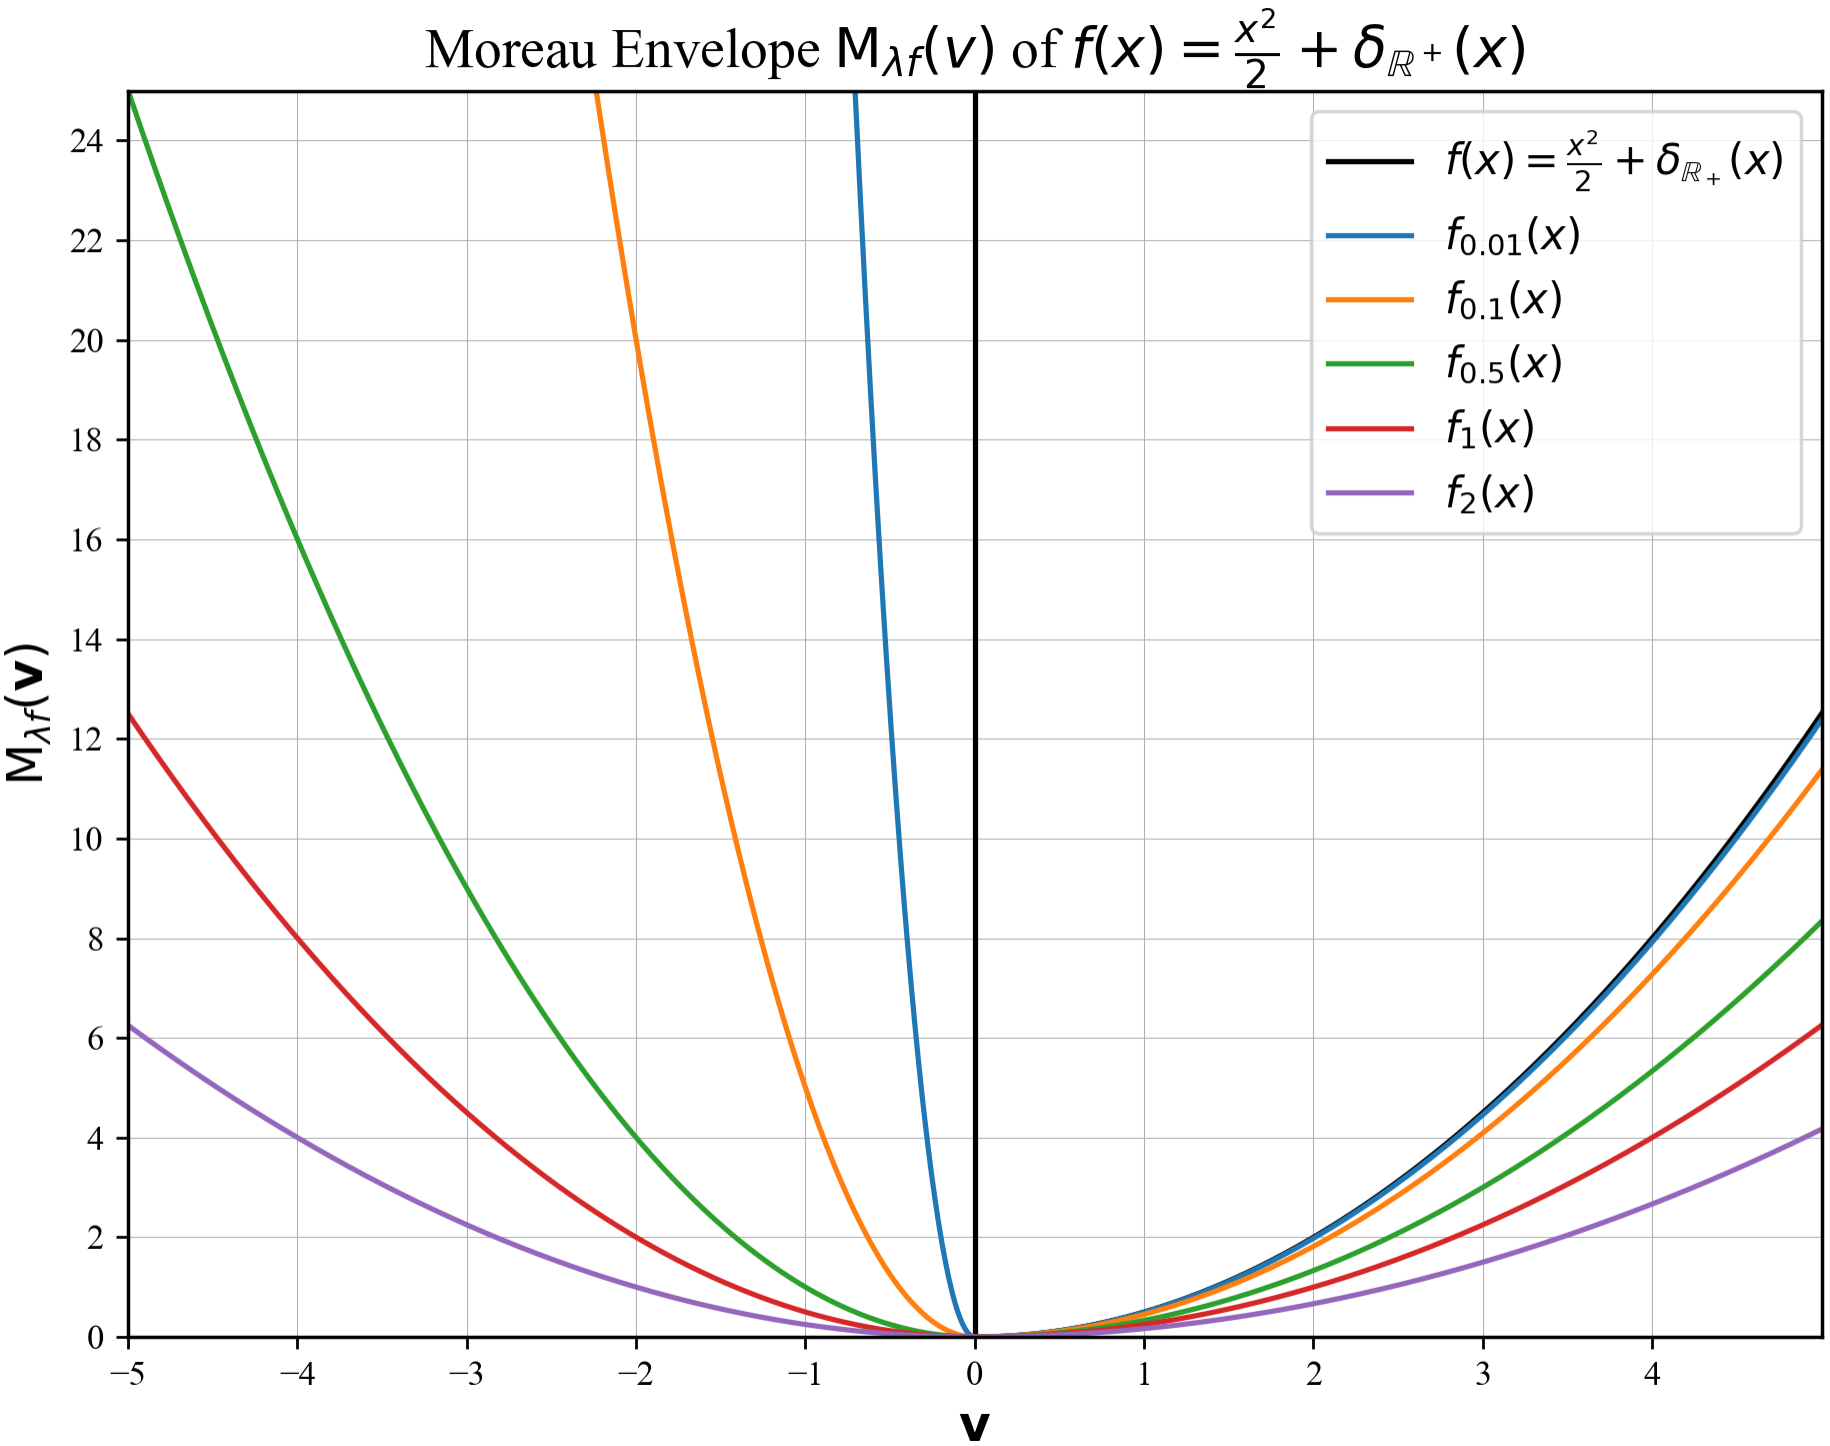
\includegraphics[width = 0.8\textwidth]{images/M_envelope.PNG}
  \caption{Moreau envelope $\mathrm{M}_{\lambda f}$ for $f = \frac{x^2}{2} + \delta_{\mathbb{R}_+}$ and different values of $\lambda$.} 
  \label{fig:moreau_envelope}
  \end{center}
\end{figure}

Figure \ref{fig:moreau_envelope} shows how $\mathrm{M}_{\lambda f}$, by adding a quadratic term to $f$ is basically a smoothed version of $f$, where the parameter $\lambda$ is a trade-off between fidelity to $f$ and smoothness. Furthermore $\mathrm{M}_{\lambda f}$ has several desirable qualities. Its domain is the whole set of real numbers $\mathbb{R}^n$, regardless of the domain of $f$. Moreover, it is continuously differentiable, even if $f$ is not, and the set of minimizers of $f$ and $\mathrm{M}_{\lambda f}$ is the same, which makes the minimization of $\mathrm{M}_{\lambda f}$ and $f$ equivalent problems. The advantage is that minimizing $\mathrm{M}_{\lambda f}$ is always a smooth problem, even though $\mathrm{M}_{\lambda f}$ can be difficult to evaluate. 

\subsubsection{Closed-form Solutions of Functions of Interest} \label{sect:prox_solutions}

\noindent\textbf{Indicator Function}

One particularly interesting case is the indicator function, for example the one given in  \eqref{eq:indicator_function}. Its proximal operator has a closed-form solution, and it is given by
\begin{equation}
\mathrm{prox}_{\lambda \delta_{\rm \mathbb{R}_+^N}}(\mathbf{v}) = \arg \min_\mathbf{x}(\delta_{\rm \mathbb{R}_+^N}+\frac{1}{2\lambda}||\mathbf{x} - \mathbf{v}||_2^2) = \arg \min_{\mathbf{x}\in \rm \mathbb{R}_+^N}\left(\frac{1}{2}||\mathbf{x} - \mathbf{v}||_2^2\right).
    \label{eq:prox_nonneg}
\end{equation}

As  \eqref{eq:prox_nonneg} demonstrates, the proximal operator of indicator functions is simply the projection from an input vector into the domain imposed by the function. For  \eqref{eq:indicator_function}, this domain is the set of real nonnegative numbers $\mathbb{R}_+^\mathrm{N}$. 

\noindent\textbf{Norms}

To evaluate the proximal operator of norms, the property known as \textit{Moreau decomposition} \cite{parikh_proximal_2014} is helpful. This property states that
\begin{equation}
\mathbf{v} = \mathrm{prox}_f(\mathbf{v}) + \mathrm{prox}_{f^*}(\mathbf{v}),
    \label{eq:moreau_dec}
\end{equation}
where $f^*$ is the conjugate function of $f$. This is very useful to evaluate proximal operators of norms, since their conjugate function is the indicator function $\mathcal{I}_{\mathcal{B}}$, where $\mathcal{B}$ is the unit ball of the norm. As aforementioned, the proximal operator of indicator functions has a closed form solution, and the problem of evaluating the proximal operator of norms reduces to evaluating the projection onto $\mathcal{B}$. Thus, \eqref{eq:moreau_dec} gives us a simple form of evaluating $\mathrm{prox}_{\lambda f}$. It follows that $\mathrm{prox}_f(\mathbf{v})$ parametrized with $\lambda$ is written as
\begin{equation}
\mathrm{prox}_{\lambda\ell_p}(\mathbf{v}) = \mathbf{v} - \lambda \Pi_{\mathcal{B}_p}(\frac{\mathbf{v}}{\lambda})
    \label{eq:norm_prox}
\end{equation}
And finding $\mathrm{prox}_{\lambda f}(\mathbf{v})$ can be done by finding $\Pi_{\mathcal{B}}(\frac{\mathbf{v}}{\lambda})$. 

Figure \ref{fig:prox_closed_form_sols} shows some element-wise plots of the closed-form solutions of functions of interest. Explicit derivations can be found in \cite{combettes_proximal_2007}. 
\begin{figure}[H]
  \begin{center}
  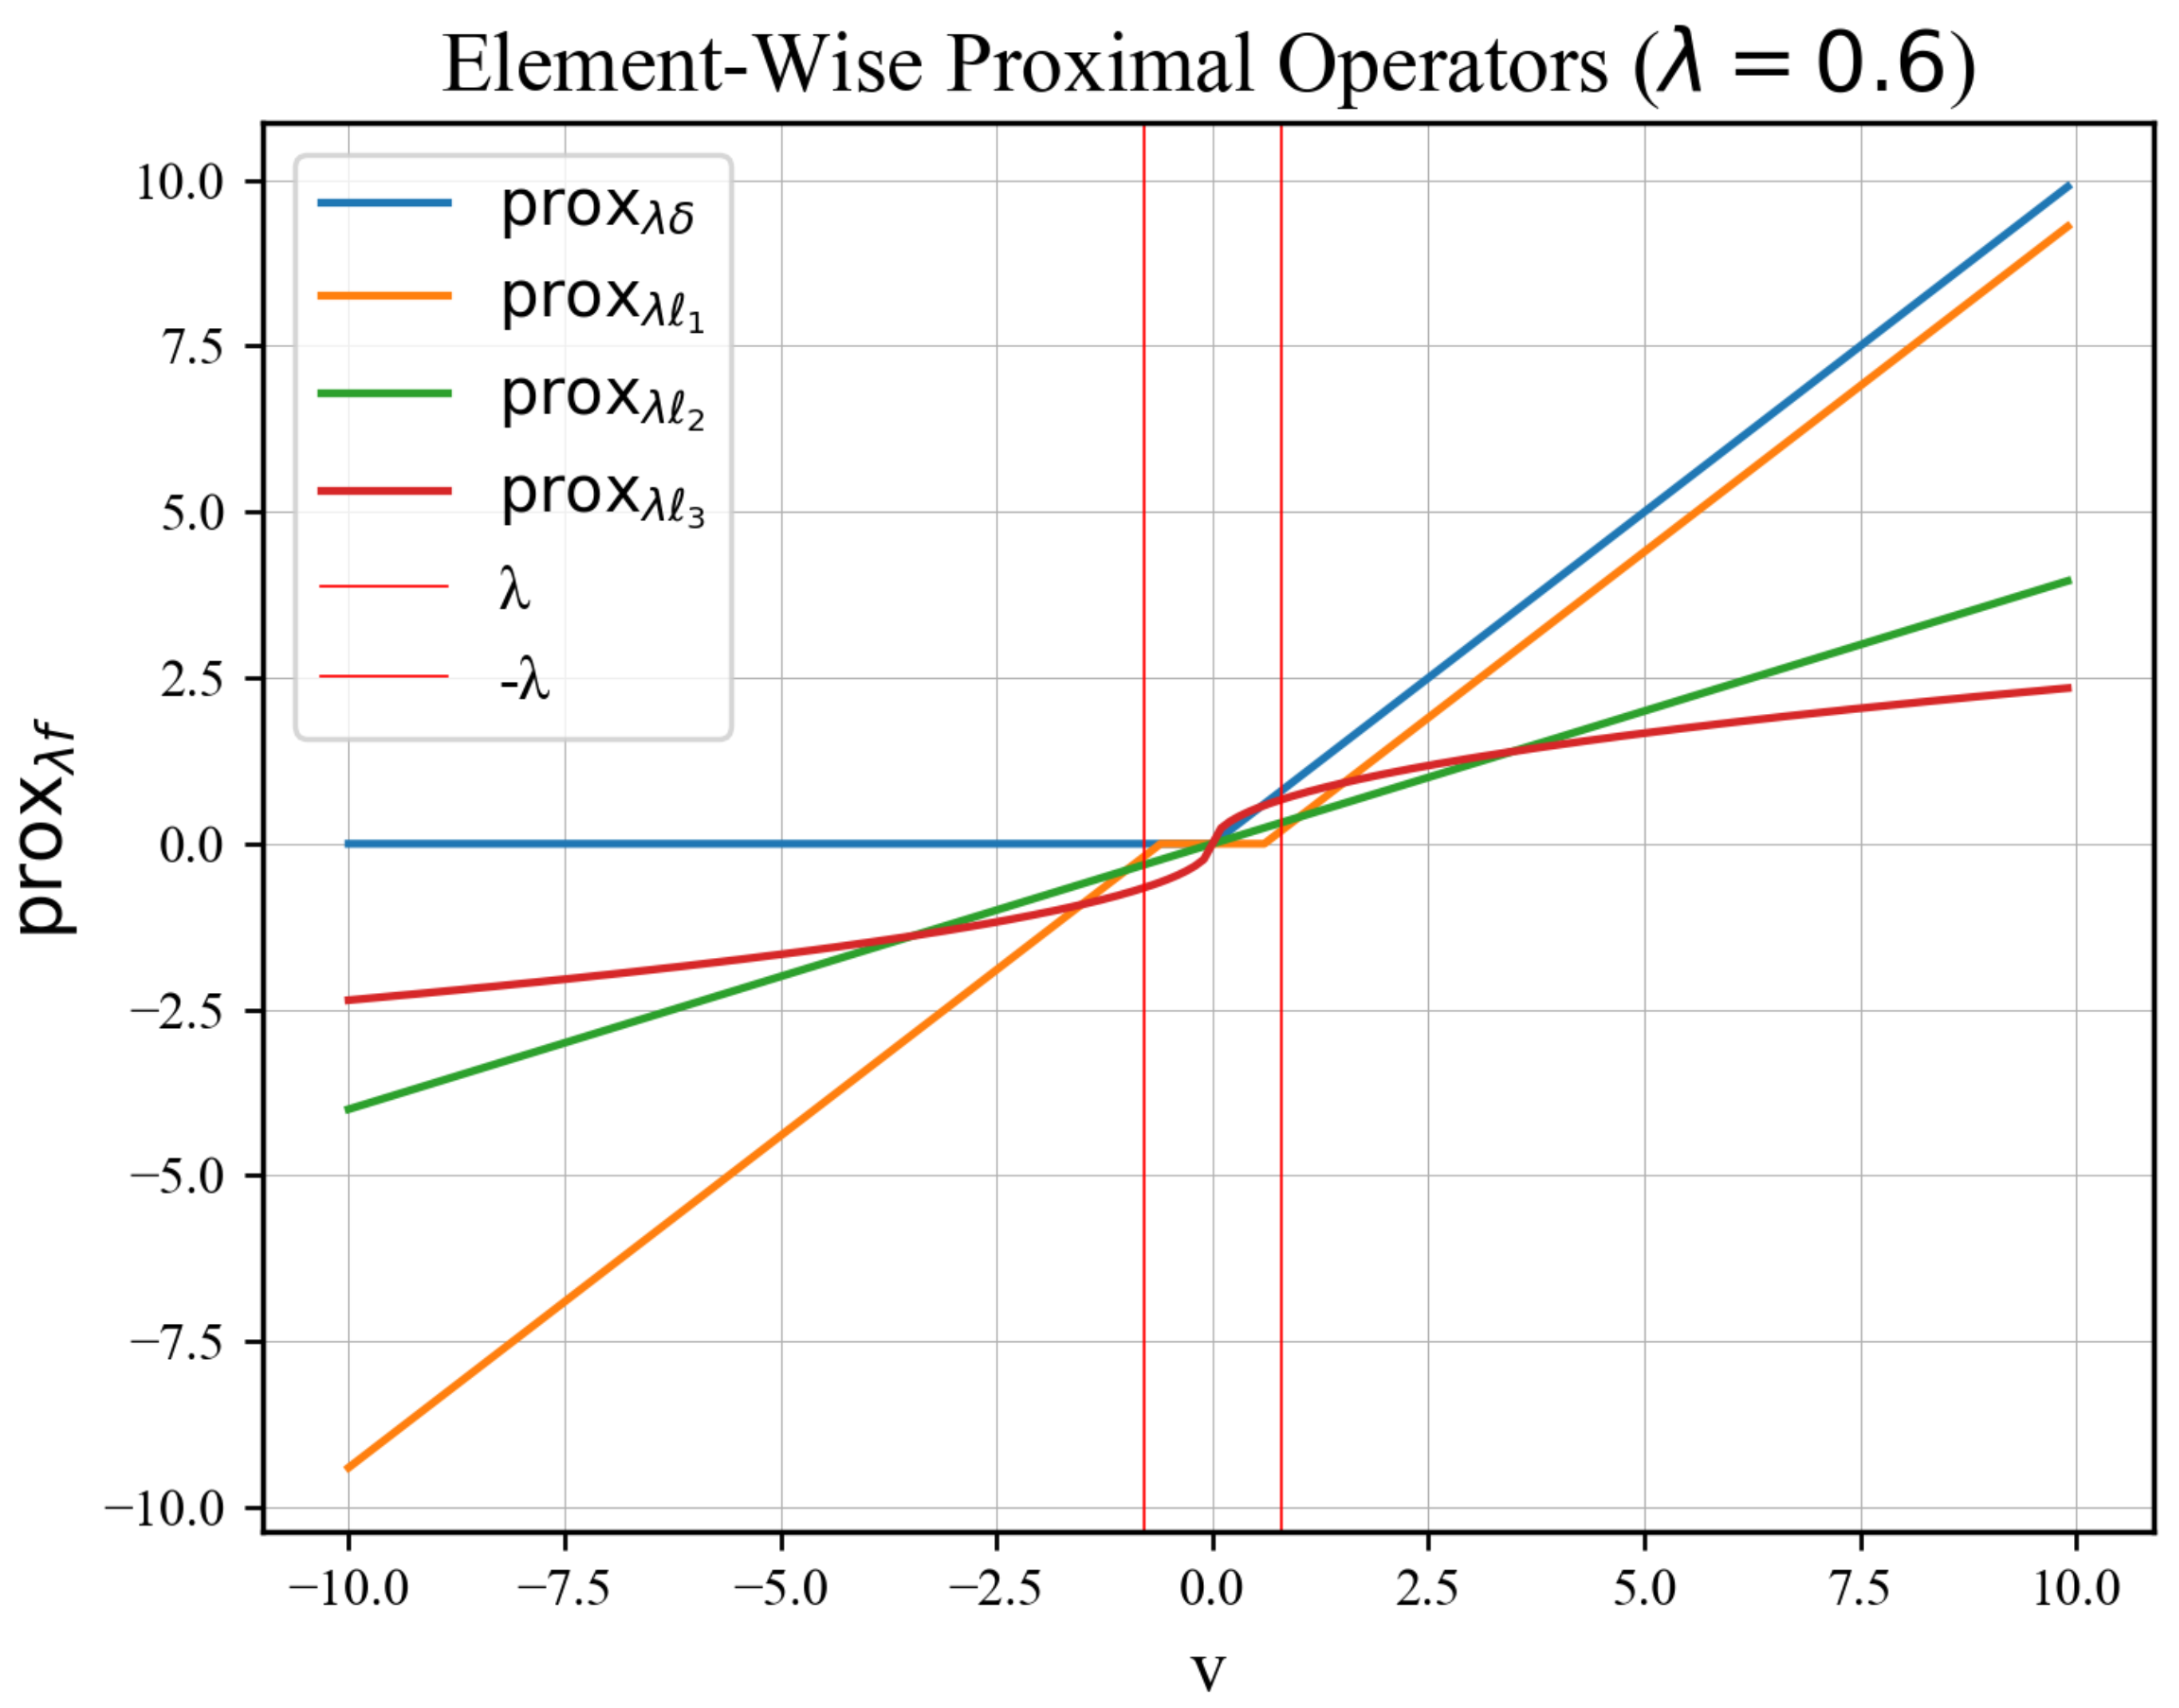
\includegraphics[width = 0.8\textwidth]{images/closed_form_sol_prox.PNG}
  \caption{Closed form solutions of element-wise proximal operators: $f = \delta_{\mathbb{R}_+^\mathrm{N}}$, $f = \ell_1$, $f = \ell_2$, and $f = \ell_3$. Note that $f = \ell_2$, and $f = \ell_3$ have been parametrized so that $\|\mathbf{v}\| = 1$.}
  \label{fig:prox_closed_form_sols}
  \end{center}
\end{figure}
In this simple functions, the effect of the proximal operator of $\ell_p$ norms and of $\delta_{\mathbb{R}_+^N}$ (defined in \eqref{eq:indicator_function}) is exemplified. For the nonnegativity constraints, where the proximal operator is the projection into $\mathbb{R}_+^\mathrm{N}$, we can see how nonnegative elements are left unchanged and negative elements are set to $0$. On the other hand, the proximal operator of the $\ell_1$ norm acts equivalently on all elements, bringing them closer to $0$ -without crossing it-, an operation called \textit{soft thresholding}. The proximal operator of the $\ell_2$ norm applies a linear transformation that depends on the value of the element $v_i$, parametrized by the norm of $\mathbf{v}$ (normalized to $1$ in Figure \ref{fig:prox_closed_form_sols}) and of course by $\lambda$. Norms of higher order have different behaviours for different values of $\mathbf{v}$, but we can see that in general they are element-wise operators.
 
% \subsubsection{Proximal Operators of Image Regularizers}

% To be included if there's time

\subsection{Proximal Optimization}

In this Section~I will describe some representative optimization algorithms that rely on the proximal operator. and are relevant in the context of image reconstruction.

\subsubsection{Example 1: Proximal Minimization}

The simplest algorithm is proximal minimization, where the update rule 
\begin{equation}
    \mathbf{x}^{k+1} := \mathrm{prox}_{\lambda f}(\mathbf{x}^k)
    \label{eq:prox_minimization}
\end{equation}
is simply applying the proximal operator on the current value.
In  \eqref{eq:prox_minimization}, $f$ is still a closed convex scalar function, $\mathbf{x}$ is the optimization variable, and $k$ is the iteration counter. One step of the proximal optimization algorithm is shown in figure \ref{fig:proximal_minimization}. 

\begin{figure}[H]
  \begin{center}
  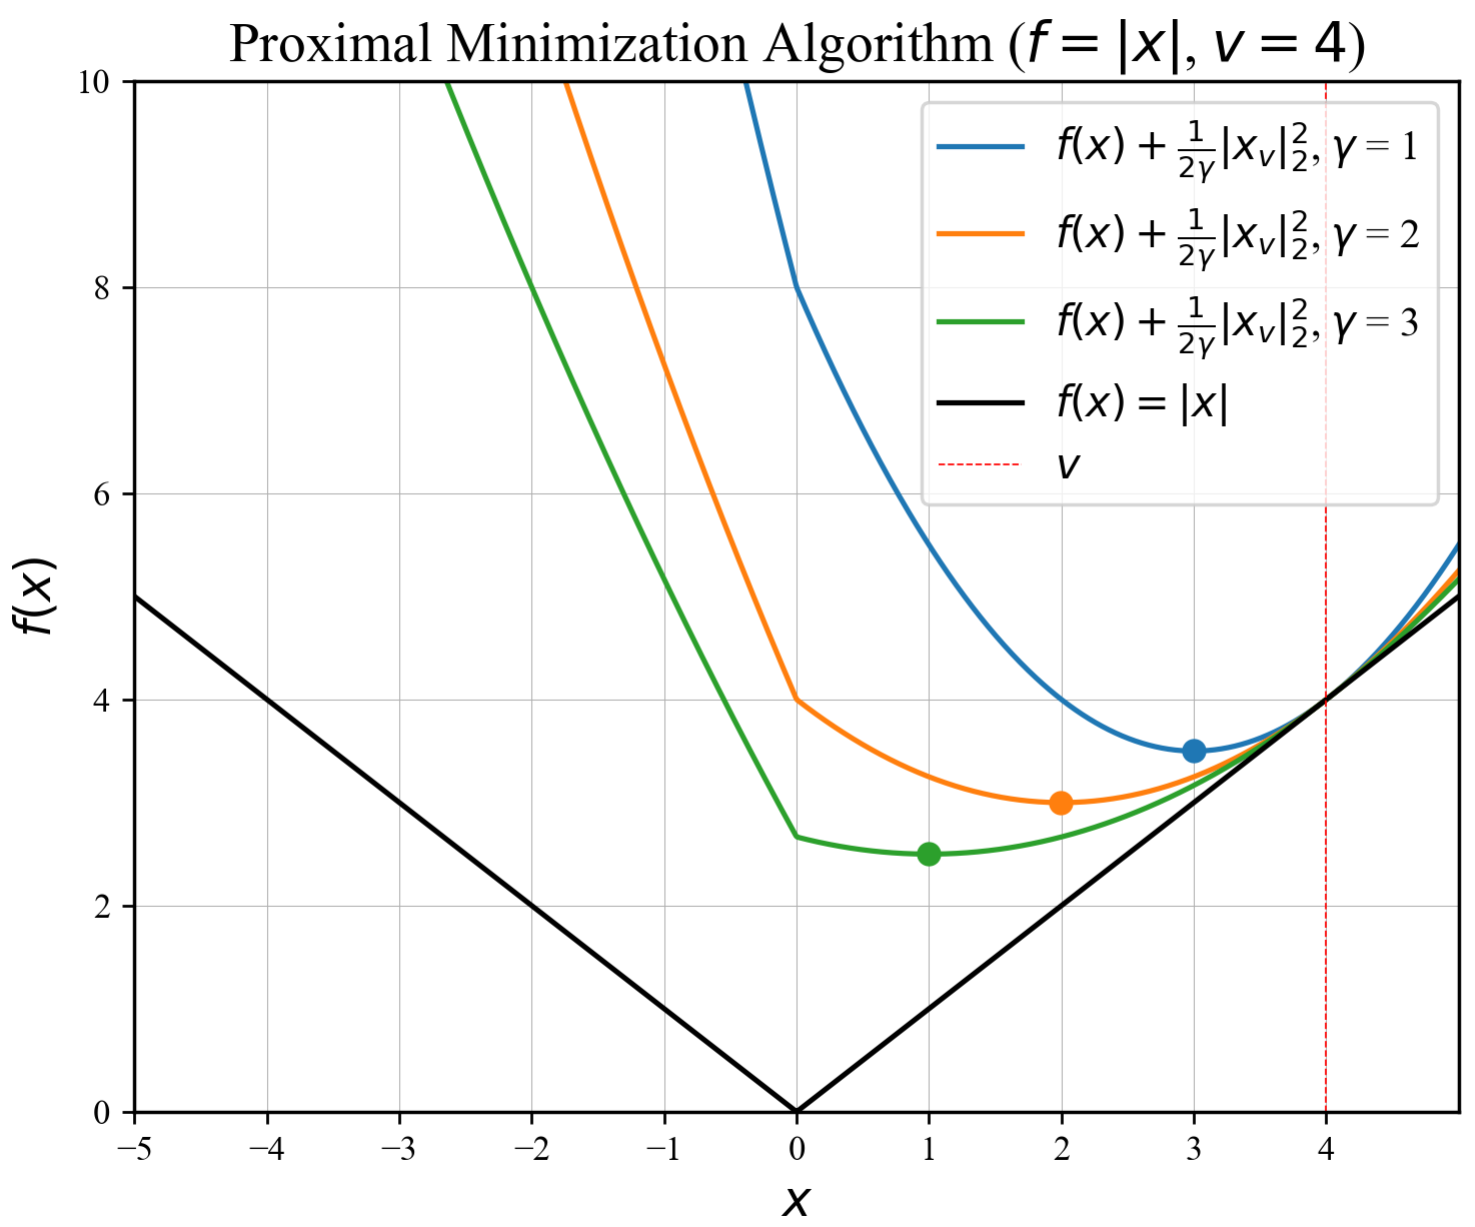
\includegraphics[scale = 0.7]{images/Proximal_minimization.PNG}
  \caption{Proximal minimization algorithm \eqref{eq:prox_minimization}. The image shows one step of the proximal minimization algorithm applied to the simple function $f(x) = |x|$ (in black). Three different values of $\lambda \in \{1, 2, 3\}$ are shown. The whole objective function is shown, and its minimum -the result of the proximal operator- is indicated in the plot.}
  \label{fig:proximal_minimization}
  \end{center}
\end{figure}

In figure \ref{fig:proximal_minimization}, the function $f(x) = |x|$ is minimized via the proximal minimization algorithm, arbitrarily choosing $v = 4$ as starting point. The objective function of the proximal operator is plotted for $\lambda \in \{1, 2, 3\}$. Note how, since $f(x)$ is the $\ell_1$ norm of a scalar, figure \ref{fig:proximal_minimization} is in complete agreement with figure \ref{fig:prox_closed_form_sols}, where it is shown the the element wise operation of $\mathrm{prox}_{\lambda \ell_1}$ is soft thresholding, with $\lambda$ as a threshold.

\subsubsection{Example 2: Proximal Gradient Method}
An algorithm that has found further applications is the \textit{proximal gradient method}. It acts on a convex objective function $f+g$, where $f: \mathbb{R}^\mathrm{N} \rightarrow \mathbb{R} $ is smooth and differentiable, but $g: \mathbb{R}^\mathrm{N} \rightarrow \mathbb{R} \bigcup \{+\infty \}$ is not. Note that since $g$ includes $\infty$ it can be the indicator function in  \eqref{eq:imaging_problem}. 

The proximal gradient method update rule is given by:
\begin{equation}
    \mathbf{x}^{k+1} := \mathrm{prox}_{\lambda g}(\mathbf{x}^k - \lambda^k \nabla f(\mathbf{x}^k)),
    \label{eq:prox_gradient_descnet}
\end{equation}
where the minimization objective is split into two, $f$ and $g$. Then, an iteration over the whole objective includes a gradient step in $f$ -note that $f$ is both smooth and differentiable- , and a a proximal minimization step in $g$. If $g$ is an indicator function, then as  \eqref{eq:prox_nonneg} shows, the minimization step over $g$ is the projection on the valid set, and the proximal gradient method becomes equivalent to projected gradient descent. %This scenario is illustrated in Figure \ref{fig:projected_grad_descent}  .

% \begin{figure}[H]
%   \begin{center}
%   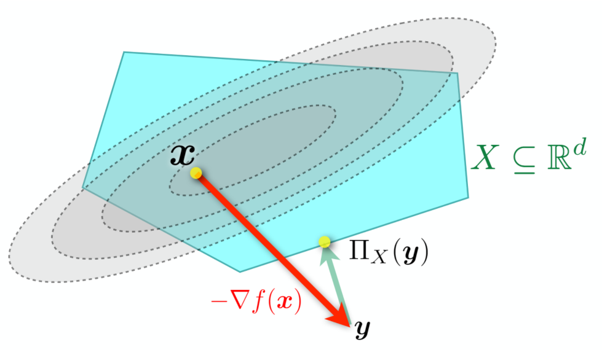
\includegraphics[width = 0.8\textwidth]{images/Projected_grad_descent.png}
%   \caption{proximal gradient method algorithm When $g$ in  \eqref{eq:prox_gradient_descnet} is an indicator function, it reduces to projected gradient mescent. Figure reuused from \href{https://github.com/epfml/OptML_course/blob/master/slides/lecture03.pdf}{CS-439 course notes}.}
%   \label{fig:projected_grad_descent}
%   \end{center}
% \end{figure}

% \begin{equation}
%     \mathrm{where}\;\;\;\; \mathbf{v} = \mathbf{x} - \lambda \nabla f(\mathbf{x})
%     \label{eq:prox_gradient_descnet}
% \end{equation}


% $\mathbf{z}_n,\; \mathbf{u}\;\in \mathbb{R}^N$

% $\mathrm{prox}_{\lambda g}, \mathrm{prox}_{\lambda f} \rightarrow$ optimization problems

\subsubsection{Example 3: ADMM} \label{sect:admm}

The alternating direction method of multipliers (ADMM) \cite{boyd_distributed_2011} is a method for minimizing objective functions of the form.
\begin{equation}
    % F_0(\mathbf{x}) + \Sigma_{n=1}^{N}F_n(\mathbf{H}_n\mathbf{x}),
    \sum_{n=1}^{N}F_n(\mathbf{H}_n\mathbf{x}),
    \label{eq:ADMM_obj}
\end{equation}
where, as before, $\mathbf{x} \in \mathbb{R}^N$, and each term of the summation has a linear operator $\mathbf{H}_n: \mathbb{R}^N \rightarrow \mathbb{R}^{Q_n}$ acting on $\mathbf{x}$ and a scalar function $F_n: \mathbb{R}^{Q_n} \rightarrow \mathbb{R}$ that has $\mathbf{H}_n\mathbf{x}$ as input. This form clearly represents \eqref{eq:imaging_problem}, since it is formed out of three separable functions, each with its own transforms and functions. For $n = 1$, the transform $\mathbf{H}_1 = \mathbf{H}$ is the forward model and $F_1 = \mathcal{D}$ is the data fidelity metric. For $n=2$, shown in \eqref{eq:regularizer}, $\mathbf{H}_2 = \mathbf{L}$ and $F_2 = \operatorname{R}$, and for $n=3$, the nonnegativity constraint, $\mathbf{H}_3 = \mathbf{I}$ is the identity operator and $F_n = \delta_{\mathbb{R}^N_+}$. Moreover, $F_n$ for all $n$ needs to be convex, but need not be neither differentiable nor smooth. Therefore, from the examples we have seen, ADMM has the broadest applicability and is one of the most relevant algorithms for image reconstruction tasks. 

The principle of ADMM is to find a saddle point of the scaled augmented Lagrangian formulation of \eqref{eq:ADMM_obj}, given by
\begin{equation}
    \mathcal{L}_{\rho}(\mathrm{\mathbf{x}},\mathbf{y}_1, …, \mathbf{y}_n,\mathbf{w}_1, …, \mathbf{w}_n) = \sum_{n=1}^N \frac12\rho_n\left\| \mathrm{\mathbf{H}_n\mathbf{x} - \mathbf{y}_n + \frac{\mathbf{w}_n}{\rho_n}}\right\|^2 + F_n(\mathrm{\mathbf{y}_n}),
    \label{eq:scaled_lag}
\end{equation}
through the update rules
\begin{equation}
    \begin{split}
    \mathbf{x}^{k+1} &:= \arg\min_\mathbf{x}\mathcal{L}_{\rho}(\mathbf{x},\mathbf{y}_1^k, …, \mathbf{y}_n^k,\mathbf{w}_1^k…\mathbf{w}_n^k)\\
    \mathbf{y}_1^{k+1} &:= \arg\min_{\mathbf{y}_1}\mathcal{L}_{\rho}(\mathbf{x}^{k+1},\mathbf{y}_1, …, \mathbf{y}_n,\mathbf{w}_1^k…\mathbf{w}_n^k)\\
    &\vdots\\
    \mathbf{y}_n^{k+1} &:= \arg\min_{\mathbf{y}_n}\mathcal{L}_{\rho}(\mathbf{x}^{k+1},\mathbf{y}_1, …, \mathbf{y}_n,\mathbf{w}_1^k…\mathbf{w}_n^k)\\
    \mathbf{w}_1^{k+1} &:= \mathbf{w}_1^k + \rho(\mathbf{x}^{k+1}-\mathbf{y}^{k+1}_1)\\
    &\vdots\\
    \mathbf{w}_n^{k+1} &:= \mathbf{w}_n^k + \rho(\mathbf{x}^{k+1}-\mathbf{y}^{k+1}_n).\\
    \end{split}
    \label{eq:admm_update}
\end{equation}
Since $\mathcal{L}_\rho$ is separable accross $n$, an update step only acts on the terms of the corresponding summation. As such, the explicit update step of $\mathbf{y}_n$ is
\begin{equation}
    \mathbf{y}_n^{k+1} := \arg\min_{\mathbf{y}_n}\left(F_n(\mathbf{y}_n) + \frac{\rho}{2} \left\|\mathbf{H}_n\mathbf{x} - \mathbf{y}_n - \frac{1}{\rho}\mathbf{w}^k_n\right\|^2 \right) = \mathrm{prox}_{ F_n\lambda}(\mathbf{x}^{k+1} - \mathbf{w}^k_n), 
    \label{eq:admm_explicit_update}
\end{equation}
Where we have made $\lambda = 1/\rho$. 

Therefore, ADMM is a common choice when the proximal operator of $f = F_n$,  $\mathrm{prox}_{ F_n\lambda}(\mathbf{v})$ is known, but the proximal operator of $f = F_n +F_{n+1}$, $\mathrm{prox}_{(F_n+F_{n+1})\lambda}(\mathbf{v})$, is not known or it is hard to evaluate, as it is the case for combinations norms with nonnegativity constraints.
% \begin{equation}
%     \begin{split}
%     \mathbf{x}^{k+1} &:= \mathrm{prox}_{\lambda f}(\mathbf{z}^k - \mathbf{u}^k)\\
%     \mathbf{z}_n^{k+1} &:= \mathrm{prox}_{\lambda g_n}(\mathbf{x}^{k+1} - \mathbf{u}^k)\\
%     \mathbf{u}^{k+1} &:= \mathbf{u}^{k+1} + \operatorname{A}\mathbf{x}^{k+1} + \operatorname{B}\mathbf{z}^{k+1}\\
%     \end{split}
%     \label{eq:prox_gradient_descnet}
% \end{equation}

% \subsubsection{Known Proximal Operators}

% Projection
% \begin{equation}
%     \begin{split}
%     \Pi_\matcal{C}(\mathbf{v}) = \arg \min_{\mathbf{x}\in \mathcal{C}}\|\mathbf{x} - \mathbf{v}\|_2
%     \end{split}
%     \label{eq:prox_gradient_descnet}
% \end{equation}

% $\mathrm{prox}_{\lambda \|\cdot \|_2}(\mathbf{v}) = \left(1 - \frac{\lambda}{\min \left( \|\mathbf{v}\|_2, \lambda \right)}\right) \mathbf{v}$

% $\mathrm{sgn}(\mathbf{x})\mathrm{max}(|\mathbf{x}| - \lambda, 0)$

% $\Pi_\matcal{C}(\mathbf{v}) = \arg \min_{\mathbf{x}\in \mathcal{C}}\|\mathbf{x} - \mathbf{v}\|_2$
\subsection{Scope of the Project} \label{sect:1.scope}

One of the drawbacks of solving an inverse imaging problem through  \eqref{eq:imaging_problem} is the splitting required to use ADMM. This splitting results in the need to optimize two additional variables of the same size of the original per extra function. Consequently, this project aims to mitigate this issue by investigating the combination of the proximal operator of common image regularizers with nonnegativity constraints. 

In other words, we will study the $\mathrm{prox}_{\lambda f}(x)$ for
\begin{equation}
    f(\mathbf{x}) = \mathcal{R}(\mathbf{x}) + \delta_{\rm \mathbb{R}_+^N}(\mathbf{x}),
    \label{eq:scope_objective}
\end{equation}
and by combination it is meant taking first the proximal of one of the two functions in $f$, then the proximal of the other function, and then check whether they are equal to $\mathrm{prox}_f$. The goal is to find regularizers for which one of the following two conditions
\begin{equation}
    \mathrm{prox}_{\mathcal{R} + \delta_{\rm \mathbb{R}_+^N}}(\mathbf{x}) =  \mathrm{prox}_{\delta_{\rm \mathbb{R}_+^N}}(\mathrm{prox}_{\mathcal{R}}(\mathbf{x}))\mbox{, or}
    \label{eq:prox_nonneg(prox_r)}
\end{equation}
\begin{equation}
    \mathrm{prox}_{\mathbb{R} + \delta_{\rm \mathbb{R}_+^N}}(\mathbf{x}) = \mathrm{prox}_{\mathcal{R}}(\mathrm{prox}_{\delta_{\rm \mathbb{R}_+^N}}(\mathbf{x}))
    \label{eq:prox_r(prox_nonneg)}
\end{equation}
are met. This has been exploited before in \cite{del_aguila_pla_cell_2018-1, del_aguila_pla_cell_2018} and the conditions for it to happen is a topic of active research in convex analysis \cite{Adly2019}.  

If, for a given regularizer, any of the two equations \ref{eq:prox_nonneg(prox_r)} and \ref{eq:prox_r(prox_nonneg)} hold, it is possible to reconstruct an image using the right-hand side of the valid equation. This means that there is no need to treat $\mathcal{R}$ and $\delta$ separately, which has the advantage of not having to store the extra variables generated during ADMM splitting. Therefore, this study has the potential of significantly reducing the computational and memory load of solving imaging problems.


